\chapter{Data Understanding}

\begin{figure}[hbtp]
	\centering
	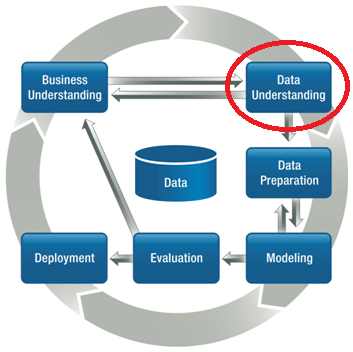
\includegraphics[width=0.5\textwidth]{./images/CRISPDM_2.png}
	\caption{CRISP-DM - Data Understanding}
	\label{CRISPDM_2}
\end{figure}

\section{Raccolta dei dati}
Il dataset preso in esame essendo oggetto della DMC 2003 Competition, è liberamente scaricabile dal sito \url{http://www.data-mining-cup.de/en/review/dmc-2003/}. 

\section{Descrizione dei dati}
Il dataset è composto da 8000 istanze rappresentanti le email. Ogni istanza è caratterizzata da 834 attributi, di cui uno \textit{target}, atto ad etichettare l'istanza come \textit{spam} o \textit{no-spam}, ed un attributo identificativo numerico (\textit{id}). Esempi di attributi utilizzati a rappresentare le istanze delle email sono le seguenti:
%Training set: 8000 Istanze 834 Attributi = 833 + Target
%data\_dmc2003\_train.txt ... 

%Test set: 11177 Istanze da classificare 833 Attributi
%data\_dmc2003\_train.txt.
\begin{table}[hbtp]
	\begin{tabular}{ c | c | c}
		\textbf{Nome attributo} & \textbf{Tipo} & \textbf{Sottotipo} \\
		\hline
		id & Categorico & Nominale \\ 
		ACCEPT\_CREDIT\_CARDS & Categorico & Nominale \\ 
		ACCOUNT\_CLICK & Categorico & Nominale \\ 
		ACT\_NOW & Categorico & Nominale \\ 
		ADDRESSES\_ON\_CD & Categorico & Nominale \\ 
		ADULT\_SITE & Categorico & Nominale \\ 
		ADVERT\_CODE & Categorico & Nominale \\ 
		ADVERT\_CODE2 & Categorico & Nominale \\ 
		ALL\_CAPS\_HEADER & Categorico & Nominale \\ 
		ALL\_CAP\_PORN & Categorico & Nominale \\ 
		ALL\_NATURAL & Categorico & Nominale \\ 
		ALTA\_BUSCADORES\_ES & Categorico & Nominale \\ 
		AMATEUR\_PORN & Categorico & Nominale \\ 
		AMAZING & Categorico & Nominale \\ 
		AMAZING\_STUFF & Categorico & Nominale \\ 
		ANOTHER\_NET\_AD & Categorico & Nominale \\ 
		AOL\_USERS\_LINK & Categorico & Nominale \\ 
		APPLY\_ONLINE & Categorico & Nominale \\ 
		APPROVED\_BY & Categorico & Nominale \\ 
		\vdots  &  \vdots  &  \vdots  \\
	\end{tabular}
\end{table}

Tutti gli attributi, ad esclusione dell'\textit{id} e del \textit{target}, sono di tipo categorico nominale booleano, esso assumerà valore 0 qualora l'email non dovesse averlo, 1 il viceversa.
Il dataset, inoltre, è distribuito in un formato testuale.


\section{Verifica della qualità dei dati}

Il dataset contiene dati di buona qualità in quanto garantiscono le seguenti qualità:

\begin{itemize}
	\item \textbf{Accuratezza}: Il dataset rispecchia perfettamente i dati reali, sono quindi da considerarsi accurati;
	\item \textbf{Completezza}: Considerati i numerosi missing values presenti, molte tuple non sono complete;
	\item \textbf{Consistenza}: I dati sono rappresentati uniformemente nella base di dati. I valori TRUE/FALSE - 0/1 - SI/NO sono stati inseriti utilizzando la sintassi TRUE/FALSE;
	\item \textbf{Attualità dei dati}: I dati sono aggiornati all'anno 2003, anno in cui è stata indetta la KDD Cup nel quale è stato utilizzato questo dataset. Il che potrebbe portare ad una classificazione errata qualora dal 2003 ad oggi, le email di spam fossero cambiate in termini di attributi caratterizzanti queste ultime.
	%Attualità dei dati: I dati non sono aggiornati al 2013 (anno attuale), ma risalgono tutti ad anni passati. Nel caso di IMDB i dati sono aggiornati al 2009, nel caso di UWCSE i dati sono aggiornati al 2004 e nel caso di WEBKB	i dati sono aggiornati al 1997. Ad ogni modo ciò non rappresenta un problema visto che l’obiettivo del KDD process è quello di valutare due versioni di un algoritmo di Data Mining.
\end{itemize}


%Bewertung der Ergebnisse
%------------------------
%
%Der Jury ist bekannt, welche von den 11.177 zu klassifizierenden
%E-Mails tatsächlich Nicht-Spam-Mail oder Spam-Mail ist. Genauer
%gesagt, stammen alle Daten aus einer Stichprobe von insgesamt
%19.177 E-Mails.
%
%Die eingesandten Ergebnisse werden mit der bekannten Information über
%die tatsächliche Zuordnung der E-Mails verglichen und der Anteil der
%nicht ausgefilterten Spam-Mails bestimmt. Gleichzeitig wird der Anteil
%der ausgefilterten Nicht-Spam-Mails ermittelt und die Einhaltung
%der 1 \% Klausel (siehe oben) überprüft. Sieger ist der Teilnehmer
%oder die Teilnehmerin, welche(r) unter Einhaltung der 1 \% Klausel die
%wenigsten Spam-Mails zustellt. Teilnehmer, die die 1 \% Klausel ver-
%letzen, werden nicht gewertet.
%
%La giuria non è noto quali classificare le e-mail è in realtà la posta o spam 11.177 non-spam. In particolare, tutti i dati provengono da un campione totale di 19.177 messaggi di posta elettronica.
%
%I risultati presentati sono confrontati con le informazioni note circa l'assegnazione effettiva delle e-mail e determinata la percentuale di spam non filtrati. Allo stesso tempo, la percentuale di filtrato non spam viene rilevato e il rispetto della clausola 1 \% (vedi sopra) selezionata. Il vincitore è il partecipante o la partecipante, che (r) manda le mail di spam in meno rispetto alla clausola 1 \%. I partecipanti, la clausola 1 \% ferire non saranno conteggiati.
%
%
%I dati contenuti nei tre database sono quasi sempre di alta qualità, ma è bene soffermarsi sulle caratteristiche che questi devono avere:
%\begin{itemize}
%	\item a;
%\end{itemize}
%
%
%Completezza: Non sempre tutti i dati sono disponibili. Ci sono alcuni missing values nei tre database.
%IMDB:nella relazione "movies" assume valore nullo l'attributo "budget" (l'informazione non è disponibile).
%UWCSE: nella relazione "persons" spesso assume valore nullo l'attributo "phase" (quando la persona è una matricola o un professore) e nella relazione "prof" talvolta assume valore nullo l'attributo "position" (non è specificata la posizione del professore). 
%Consistenza: I dati sono rappresentati uniformemente nella base di dati. I valori TRUE/FALSE - 0/1 - SI/NO sono stati inseriti utilizzando la sintassi TRUE/FALSE in tutti i database. 
%Attualità dei dati: I dati non sono aggiornati al 2013 (anno attuale), ma risalgono tutti ad anni passati. 
%Nel caso di IMDB i dati sono aggiornati al 2009, nel caso di UWCSE i dati sono aggiornati al 2004 e nel caso di WEBKB i dati sono aggiornati al 1997. Ad ogni modo ciò non rappresenta un problema visto che l’obiettivo del KDD process è quello di valutare due versioni di un algoritmo di Data Mining.Non sono richiesti dati esterni da integrare nelle tre basi di dati.

\section{Esplorazione dei dati}
I dati essendo dei valori booleani indicando la presenza/assenza della feature per quel dato, sono da considerarsi di tipo categorico nominale; Il che porta a poter utilizzare solo grafici in grado di rappresentare la frequenza con cui una feature è presente sui dati. A tale scopo, verranno utilizzati essenzialmente degli istogrammi sugli attributi aventi meno missing value.

\begin{figure}[hbtp]
 	\centering
 	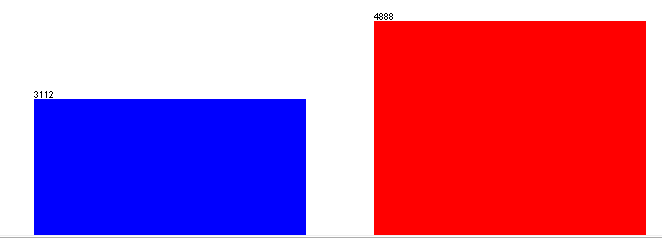
\includegraphics[width=0.4\textwidth]{./images/histogram/target.png}
 	\caption{Istogramma attributo Target}
 	\label{TargetHist}
\end{figure}

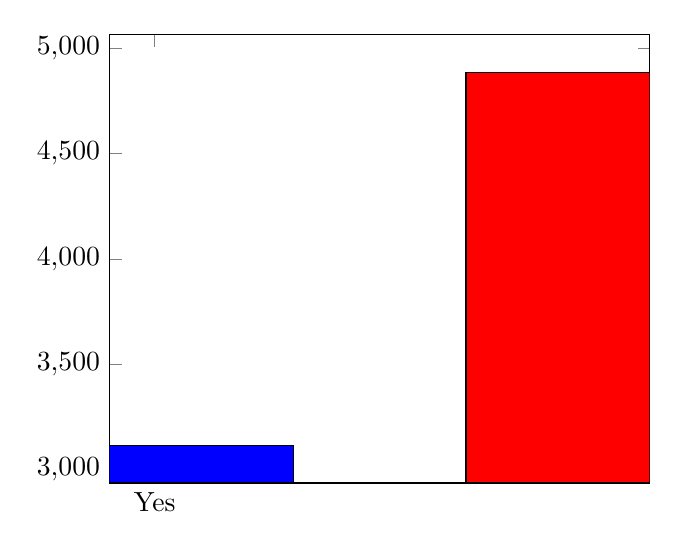
\begin{tikzpicture}
  \begin{axis}[
  symbolic x coords={Yes,No},
  xtick=data,
  bar width=100pt,
  ]
  \addplot[ybar,fill=blue] coordinates {
  	(Yes,   3112)
  };
  \addplot[ybar,fill=red] coordinates {
  	(No,   4888)
  };
  \end{axis}
  \end{tikzpicture}
  
 %TODO Fare instogrammi in latex
